\chapter{Economics \small{\textsf{DRAFT}}}\label{chapter:economics}

\section{Our Variables}
\begin{itemize}
    \item $\kappa$: security parameter
    \item $\mathcal{A}$: adversary
    \item $H$: hash
    \item $T$: target
    \item $p$: prob of successful query
    \item $n$: total parties
    \item $t$: adversarial parties
    \item $q$: hash rate
    \item $k$: common prefix
    \item $\mu$: Chain Quality
    \item $\tau$: Chain Growth
\end{itemize}

\section{Some Bitcoin Statistics}
We can take a look at the blockchain statistics for Bitcoin on the website:\\
\href{https://www.blockchain.com/charts/hash-rate}{https://www.blockchain.com/charts/hash-rate}.
Today, the hash rate of the bitcoin network is $210.48$m TH/s, measured in terahertz per second, as shown in Figure ~\ref{fig:hash_rate}. This can be denoted as:
\begin{align*}
    q\cdot (n-t) \approx 2^{67} \texttt{ Hz}.
\end{align*}


\begin{figure}[ht]
    \centering
    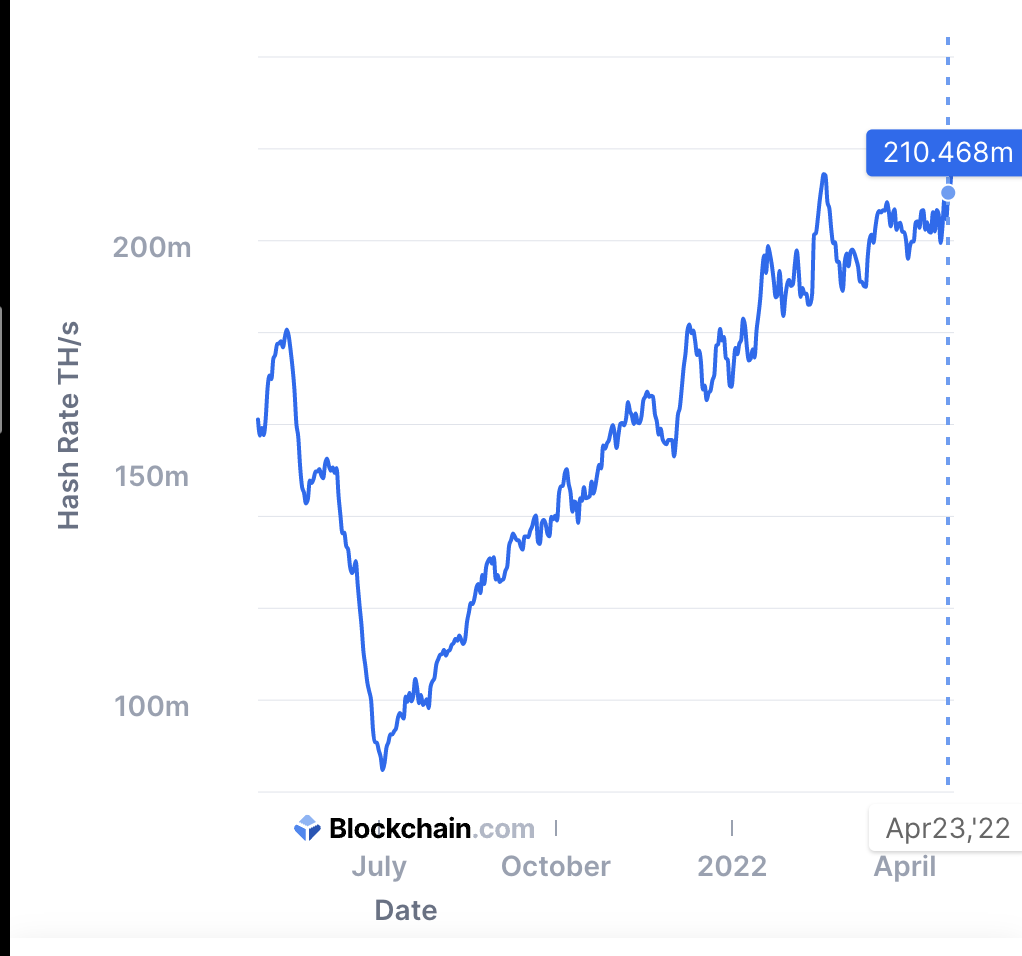
\includegraphics[scale = 0.6]{figures/hash_rate.png}
    \caption{Hash Rate of Bitcoin from April 2021 to April 2022\cite{hash-rate}}
    \label{fig:hash_rate}
\end{figure}

We can estimate the value of $q$ (the hash power of 1 party) on a real computer. On a laptop, $q \approx 100 \texttt{MHz}$. On a GPU, we can raise this to $q \approx 20 \texttt{ GHz}$. Today, we also use specialized mining power, with the best machines (ASICs) achieving $q \approx 200 \texttt{ THz}$. To see the hash power of the ASIC machine, you can refer to this website: \href{www.asicminervalue.com}{www.asicmine
rvalue.com}

We can also use the website to examine the number of transactions that are confirmed in any time frame. Here are some other observations:
\begin{itemize}
    \item The number of transaction spikes in the weekdays and toughs on the weekends
    \item The number of UTXOs grew significantly in the past year
    \item The mempool size is more erratic
\end{itemize}
Overall, observe that many network activity values depend on human factors.

\section{Mining}
\subsection{Parties}
In the world of blockchain, there are parties that are not honest. We would like at least the majority of parties to be honest for our blockchain system to work well, so to encourage honesty it should be disadvantageous to be an adversarial party. In addition, we make the assumption that the members of the honest majority generally act rationally with respect to what is most beneficial economically. Our goal is that for the honest parties to maximize their profits, they should behave in a predictable, rational manner.

\begin{figure}[ht]
    \centering
    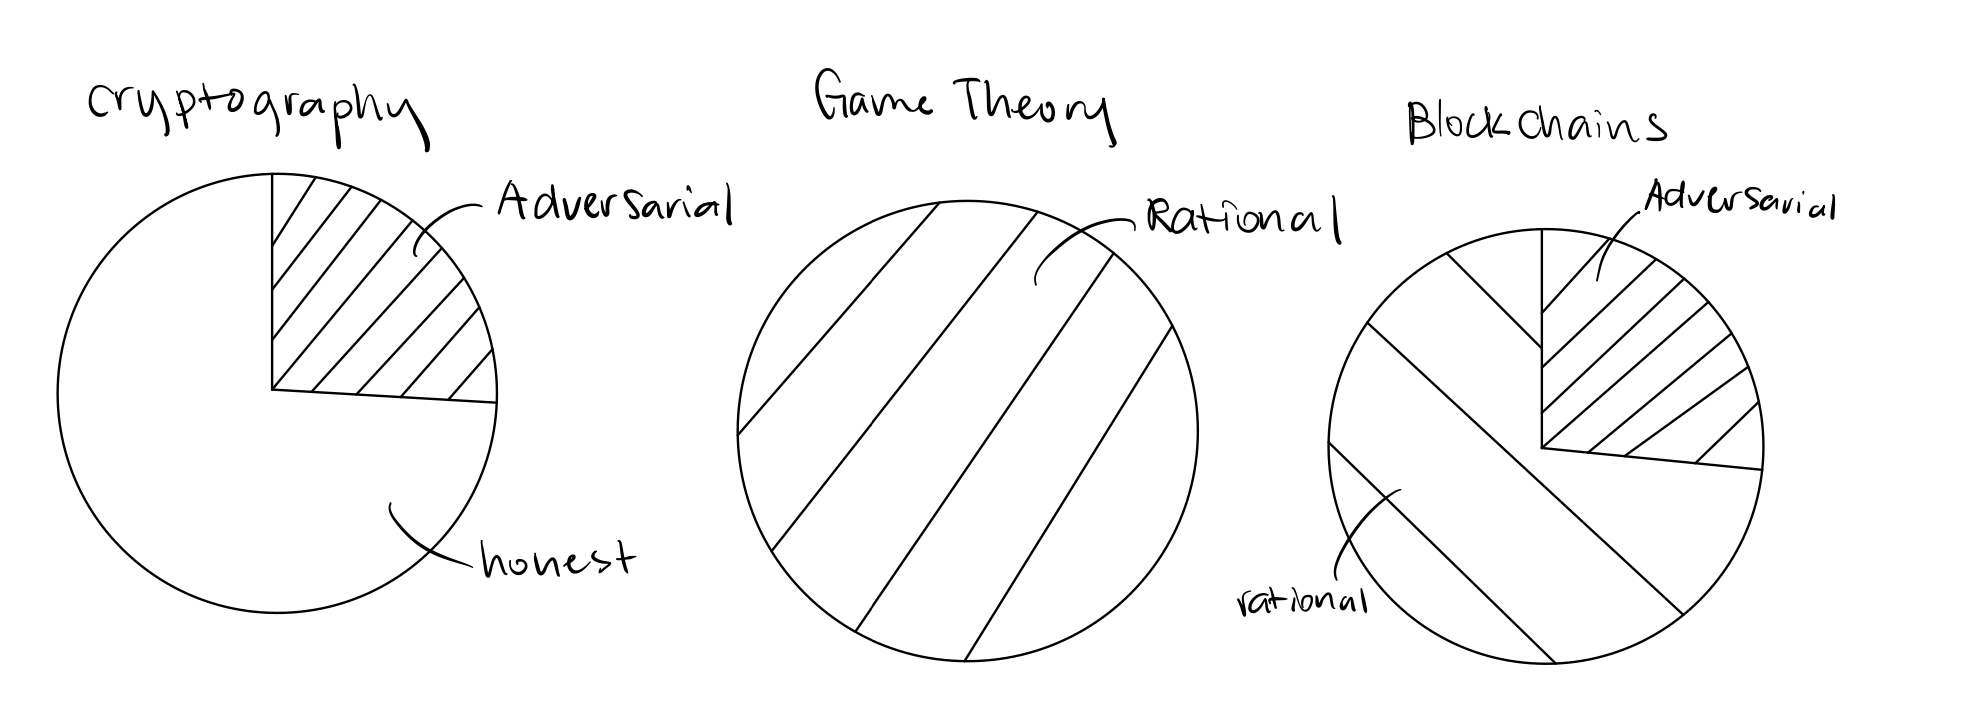
\includegraphics[scale = 0.4]{figures/rational.png}
    \caption{Types of Parties in Cryptography, Game Theory, and Blockchains}
    \label{fig:rational}
\end{figure}

However, for blockchain, we assume that the users consist of adversarial and rational parties.

\subsection{The parameter $\Delta$ and Block Size Limit}
Previously, we defined $\Delta$ as the parameter for the network delay, which is also the desired parameter for the average time of block mining. From the previous lectures, we may assume that $\Delta$ is a constant. However, in practice, as more transactions gets placed into a block, the size of the block increases, so the time it takes for the entire network download the block also increases. Since we would like network delay to be lower than a small fixed value, in practice blockchains have a block size limit specifying the maximum size in bytes of a block.

\subsection{Including a transaction}
Now that we have a constraint on the block size, the rational miner should adopt some strategies to maximize profit. Difference combinations of transactions in a block will give different rewards, so a rational miner should choose carefully which transactions to include in a block. When putting together a new block to mine, a miner will encounter one of two cases:

\begin{quote}
    Case 1: Mempool fits in block $\longrightarrow$ include all transactions to the new block

    Case 2: Mempool does not fit $\longrightarrow$ sort transactions by their fee-per-byte and include the top transactions until the block reaches the size limit
\end{quote}

Case 1 is easy, but Case 2 can be reduced to the knapsack problem, which is NP-hard. Furthermore, transaction ordering is affected by extra constraints: we have to order the transactions in a block such that if a transaction spends the output of another transaction in the mempool, it must appear after the transaction it spends in the block. The actual way transactions are selected are implementation details which are decided by each miner. In any case, since transaction fees provide extra reward, a rational miner would not mine an empty block.

Since miners prefer to mine more profitable transactions (i.e. those with higher fees), the chosen transaction fee would determine the confirmation time for a transaction. If a wallet wants their transaction to be confirmed faster, they would set a higher fee to incentivize miners to include the transaction into their blocks. If the wallet pays a lower fee, the transaction may take longer to be included, or never be included.

\subsection{Block Reward}
Previously, we defined the coinbase value as:
\begin{align*}
    \text{Coinbase value} &= \text{block reward + fees}
\end{align*}
In the Marabu protocol, the block reward is fixed. However, in Bitcoin and many other real-world cryptocurrencies, the block reward decreases over time. Bitcoin implements a macro-economic policy called ``reward halving", shown in Figure \ref{fig:reward_halving}, in which the block reward is halved every 4 years. The sum is finite, thus the supply of bitcoin is finite, at around 21 million total.

\begin{figure}[ht]
    \centering
    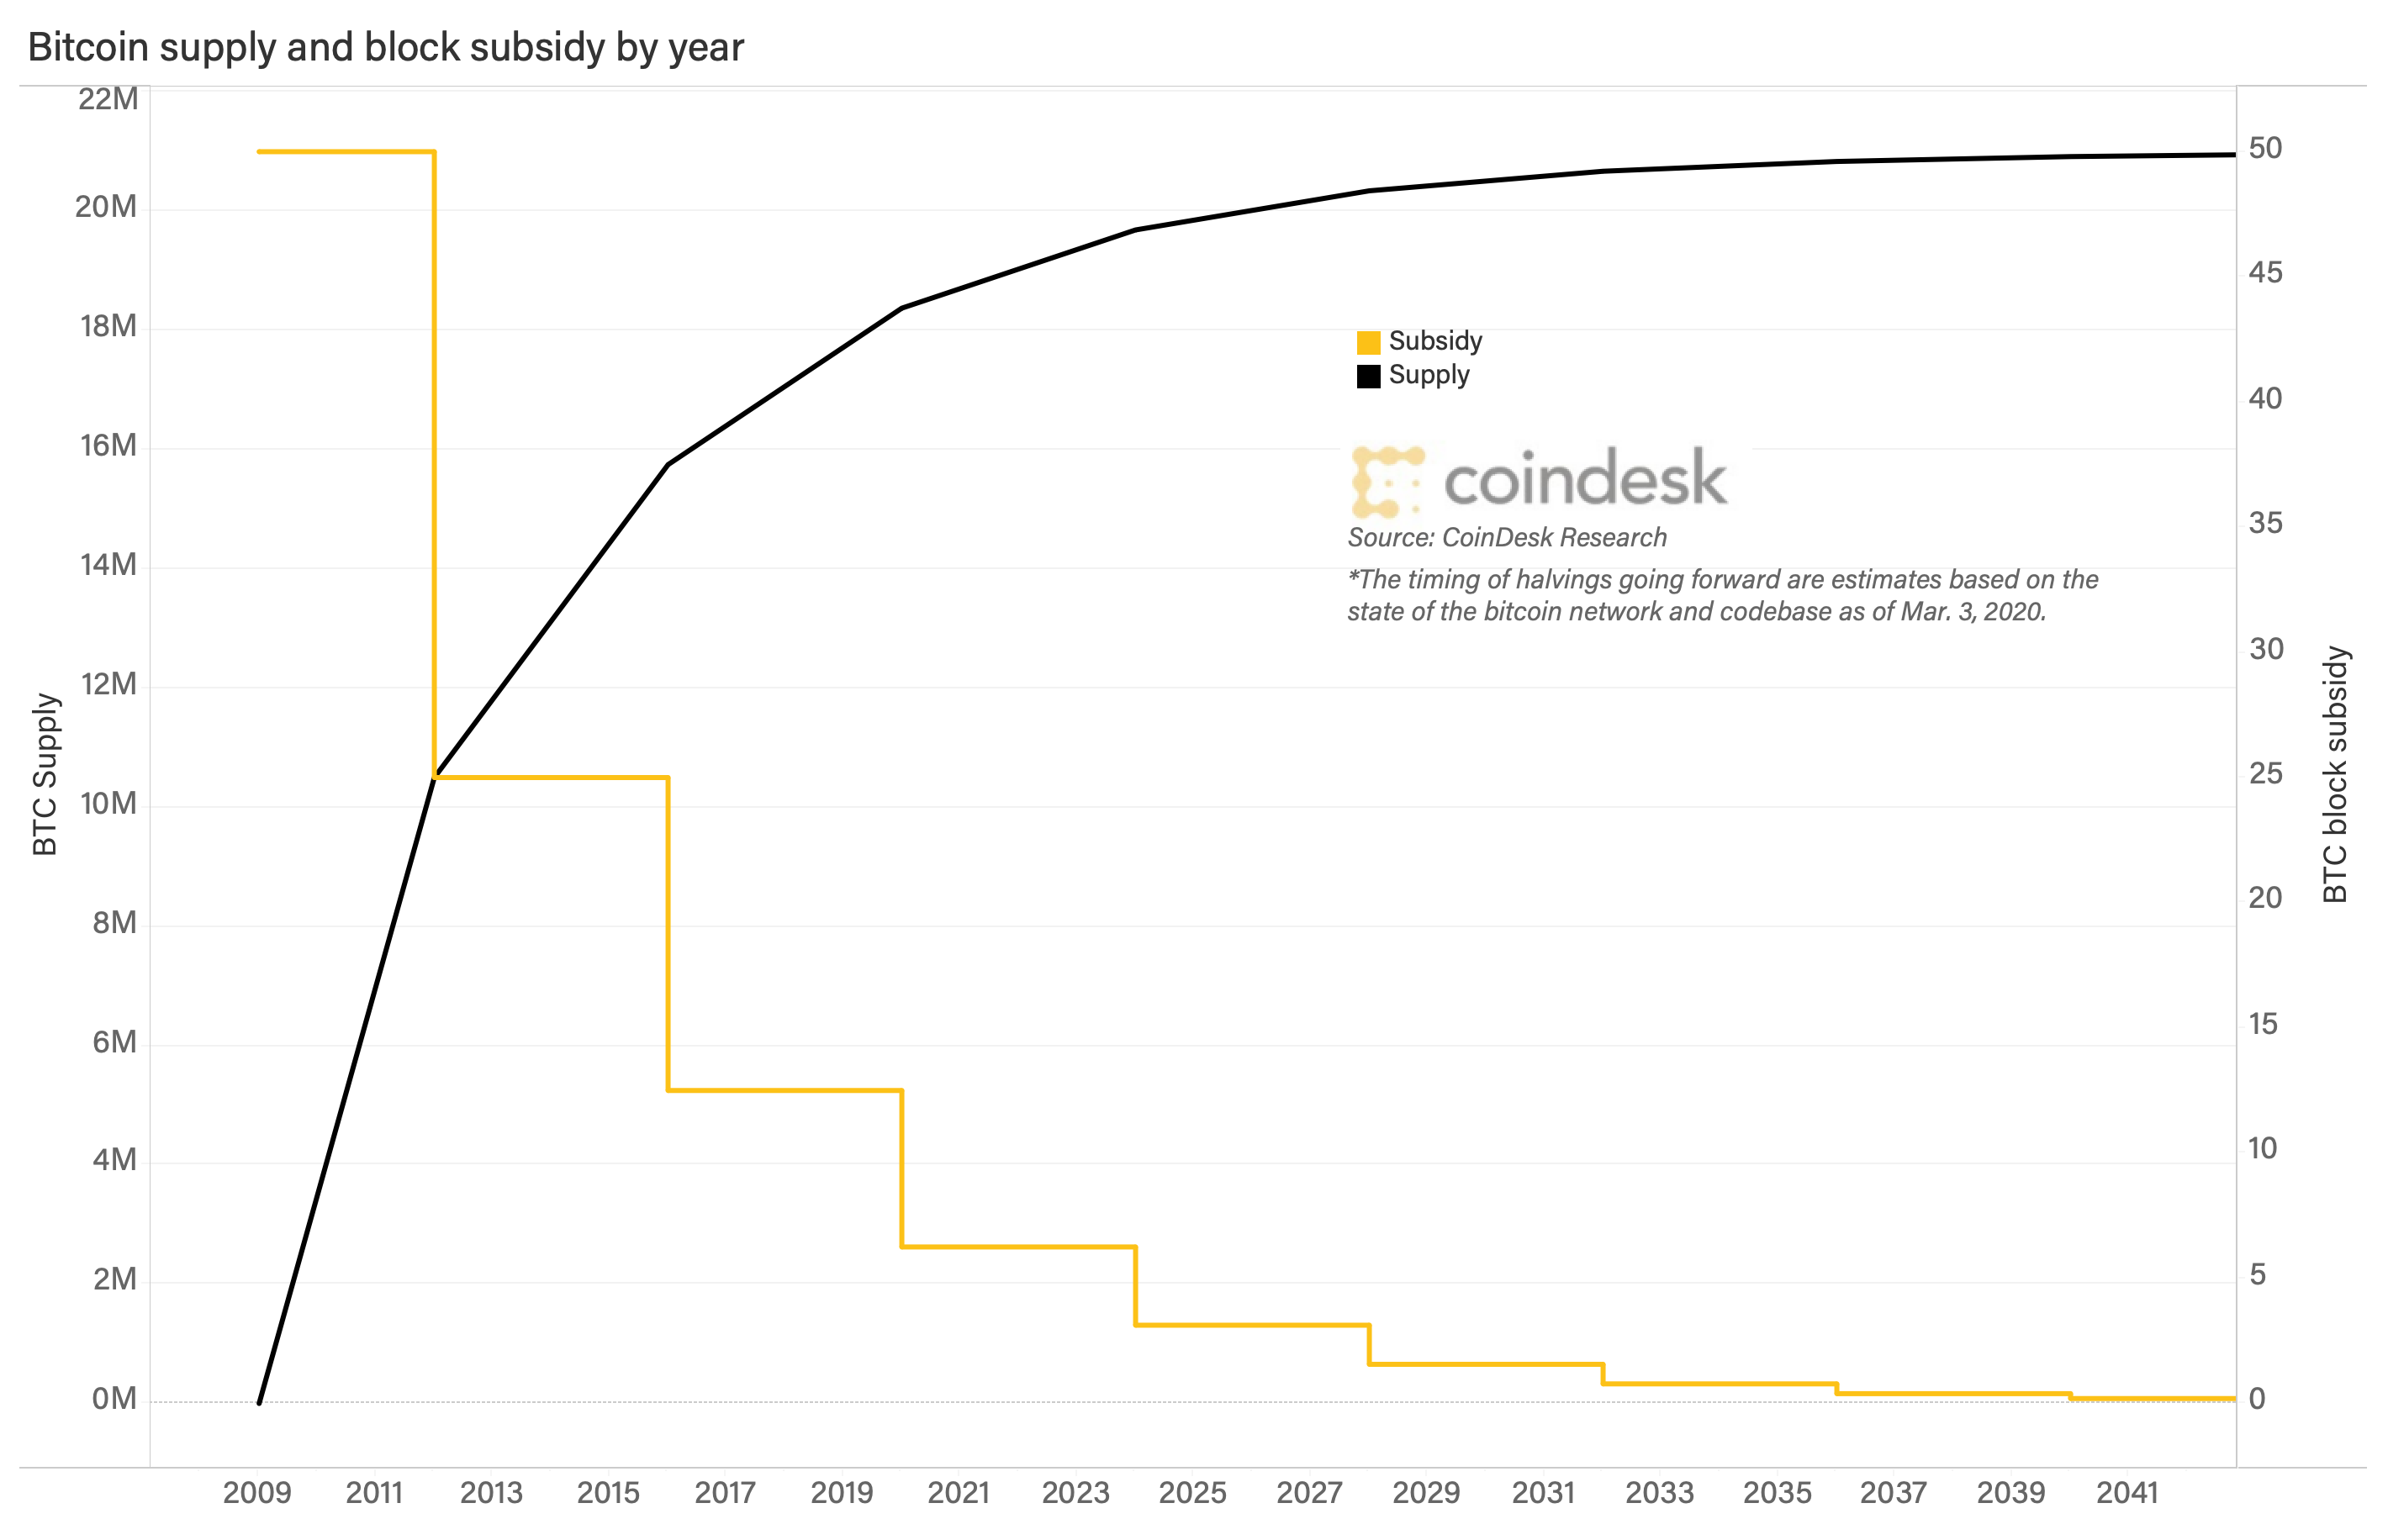
\includegraphics[scale = 0.2]{figures/reward_halving.png}
    \caption{Reward Halving for Bitcoin Supply\cite{halving}}
    \label{fig:reward_halving}
\end{figure}

Other implementations of cryptocurrencies, such as Monero, have also chosen a smooth emissions where the change of the block reward is continuous, and the sum still converges to a constant.


\section{Variable Mining Difficulty}
The Marabu protocol has a constant difficulty parameter, and thus a constant target $T$. However, this creates a problem since the hash power of the network is constantly changing. Therefore, when the hash power increases, the rate of block production could be less than $\Delta$. To keep a desired block production rate, we want to scale the difficulty appropriately as the hash power of the network increases.

\subsection{Definitions}

\begin{definition}
    Let $f$ be the probability of getting an honest block in one unit of time. Then,
\begin{align*}
    f &\approx p \cdot q \cdot (n-t) \\
    f &= 1- (1-p)^{q(n-t)}
\end{align*}
where $(1-p)^{q(n-t)}$ is the probability that every honest party failed.
\end{definition}
In Bitcoin, where 1 block is produced approximately every 10 minutes, we have $f \approx 1/600$ seconds. For small $p$, we have
\begin{align*}
    (1-p)^{q(n-t)} \approx 1 - qp(n-t)
\end{align*}

\begin{definition}
Let $\eta = \frac{1}{f}$ be the expected block production duration.
\end{definition}
We split the chain into sections $m$ blocks long.
\begin{definition}
Let an \textit{epoch} be a section that is $m$ blocks long, where $m$ is a constant.
\end{definition}
Given the target for epoch $j-1$, denoted $T_{j-1}$, we wish to find the target for the next epoch $T_j$. The desired epoch duration is $m\cdot \eta$, the number of blocks times the expected production rate, but the actual duration is $t_2-t_1$ where $t_1$ and $t_2$ gives the mining times of the first and last blocks of the epoch $j-1$, respectively. Then we recalculate the target via

\begin{align*}
    T_j = T_{j-1}\frac{t_2 - t_1}{m\eta}
\end{align*}

We reach the following conclusion:
\begin{quote}
If actual time $<$ desired $\longrightarrow$ target decreased, difficulty increased.\\
If actual time $>$ desired $\longrightarrow$ target increased, difficulty decreased
\end{quote}

\section{Mining Pools}
The probability of an individual miner successfully mining a block (and earning \$200k for the reward) is low. This reward has a high expectation, but it also has high variance. However, the miners want a consistent return, with the same expectation but a lower variance. To do this, miners combine together to form a \textit{pool}.

\begin{definition}
A \textit{pool} is a collaboration of miners. If any one miner succeeds, then they share the profit with other miners.
\end{definition}

\subsection{How Pools Work}
The pool operator, a trusted party, generates a key pair ($pk, sk$) and shares the public key $pk$ with all miners. The participants mine the block, in which the coinbase transaction goes to the public key $pk$ of the pool operator. Then, the operator distributes profits to the miners.

Now the pool operator must verify that the miners are actually mining. They could achieve this by setting up a light PoW verification.
\begin{definition}
The \textit{light PoW} equation provides a target that is significantly easier, called a \textit{light block share}:
\begin{align*}
H(B) &\leq 2^\xi T
\end{align*}
where $\xi$ denotes a constant that scales the target.
\end{definition}
The participants would send the light PoW block to the operator once they have mined a block. The operator validates that:
\begin{enumerate}
    \item The light block share satisfied the light PoW equation
    \item The coinbase pays the operator\end{enumerate}

Finally, after the block is mined, the operator distributes profits in proportion to the shares reported. An adversarial miner can only get payed if they submit the valid light block share. Additionally, the miner cannot change a valid block's public key to their own address because this will change the hash. Finally, an adversary would want to share a found block because they would get rewarded as part of the pool.

\section{Wallets}

\subsection{Mining and Wallets}
While miners wish to maximize fees to increase their rewards, wallets wish to minimize fees to decrease the price of transactions. The fee-per-byte is fixed by the user, so one way to lower the transaction fee is to minimize the size in bytes of the transaction. In case a user miscalculates the fee-per-byte and gives a value that is too low, an honest user can submit the same transaction but with a higher fee. This is an ``honest" double spend called a \textit{replace by fee}, as shown in Figure \ref{fig:replace_by_fee}. The higher-fee transaction replaces the older one in the mempool.

\begin{figure}[ht]
    \centering
    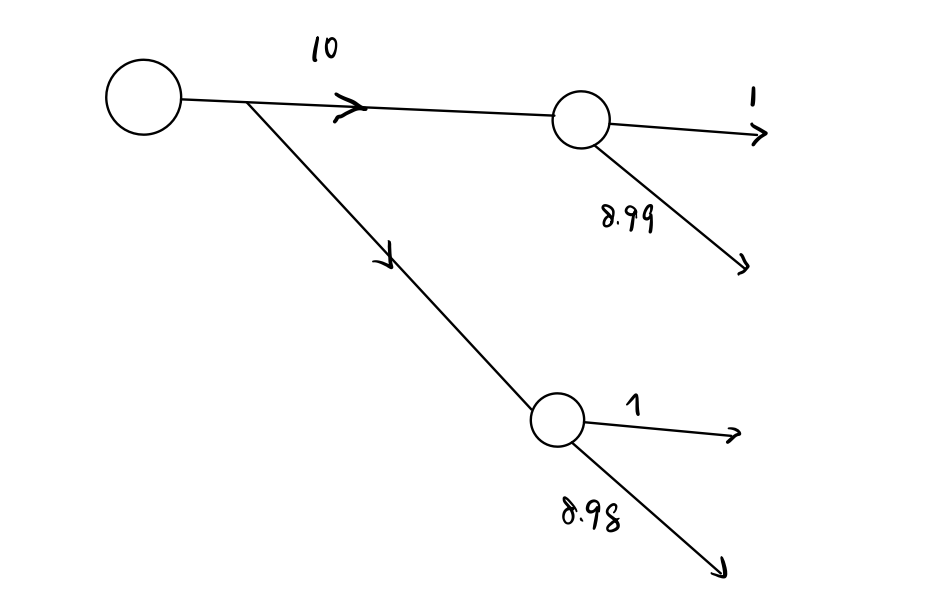
\includegraphics[scale = 0.5]{figures/replace_by_fee.png}
    \caption{An example of a honest, rational party not being able to send a transaction and creating another replace by fee transaction}
    \label{fig:replace_by_fee}
\end{figure}


\subsubsection{Types of Wallets}
Wallets can be ``hot" or ``cold". Hot wallets are online, so they are easily available to use but less secure. Cold wallets are stored offline, such as in a hardware wallet or written down on a piece of paper. The hardware wallet could be plugged into a computer. The computer would store the transaction information, while the wallet generates the public keys, secret keys, and the signature without the secret keys leaving the device. They are more secure but tend to be harder to operate.


\begin{figure}[ht]
    \centering
    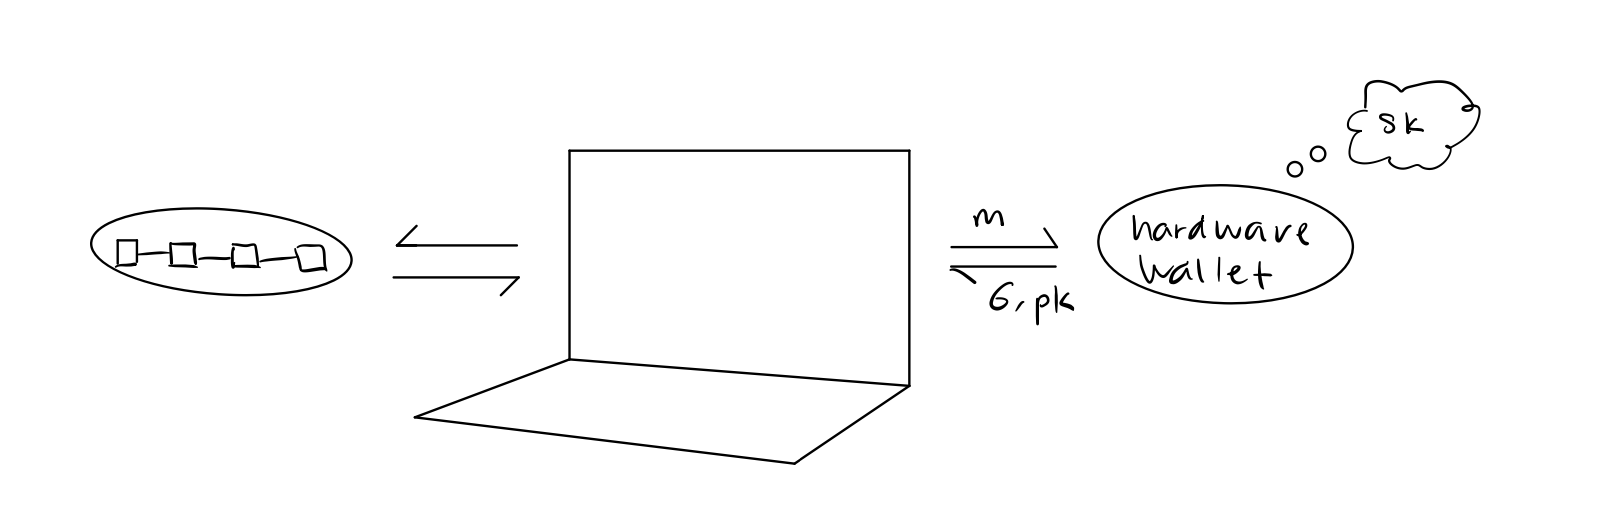
\includegraphics[scale = 0.5]{figures/hardware.png}
    \caption{Illustration of the interactions between the hardware wallet and the computer}
    \label{fig:hardware}
\end{figure}

\begin{figure}[ht]
    \centering
    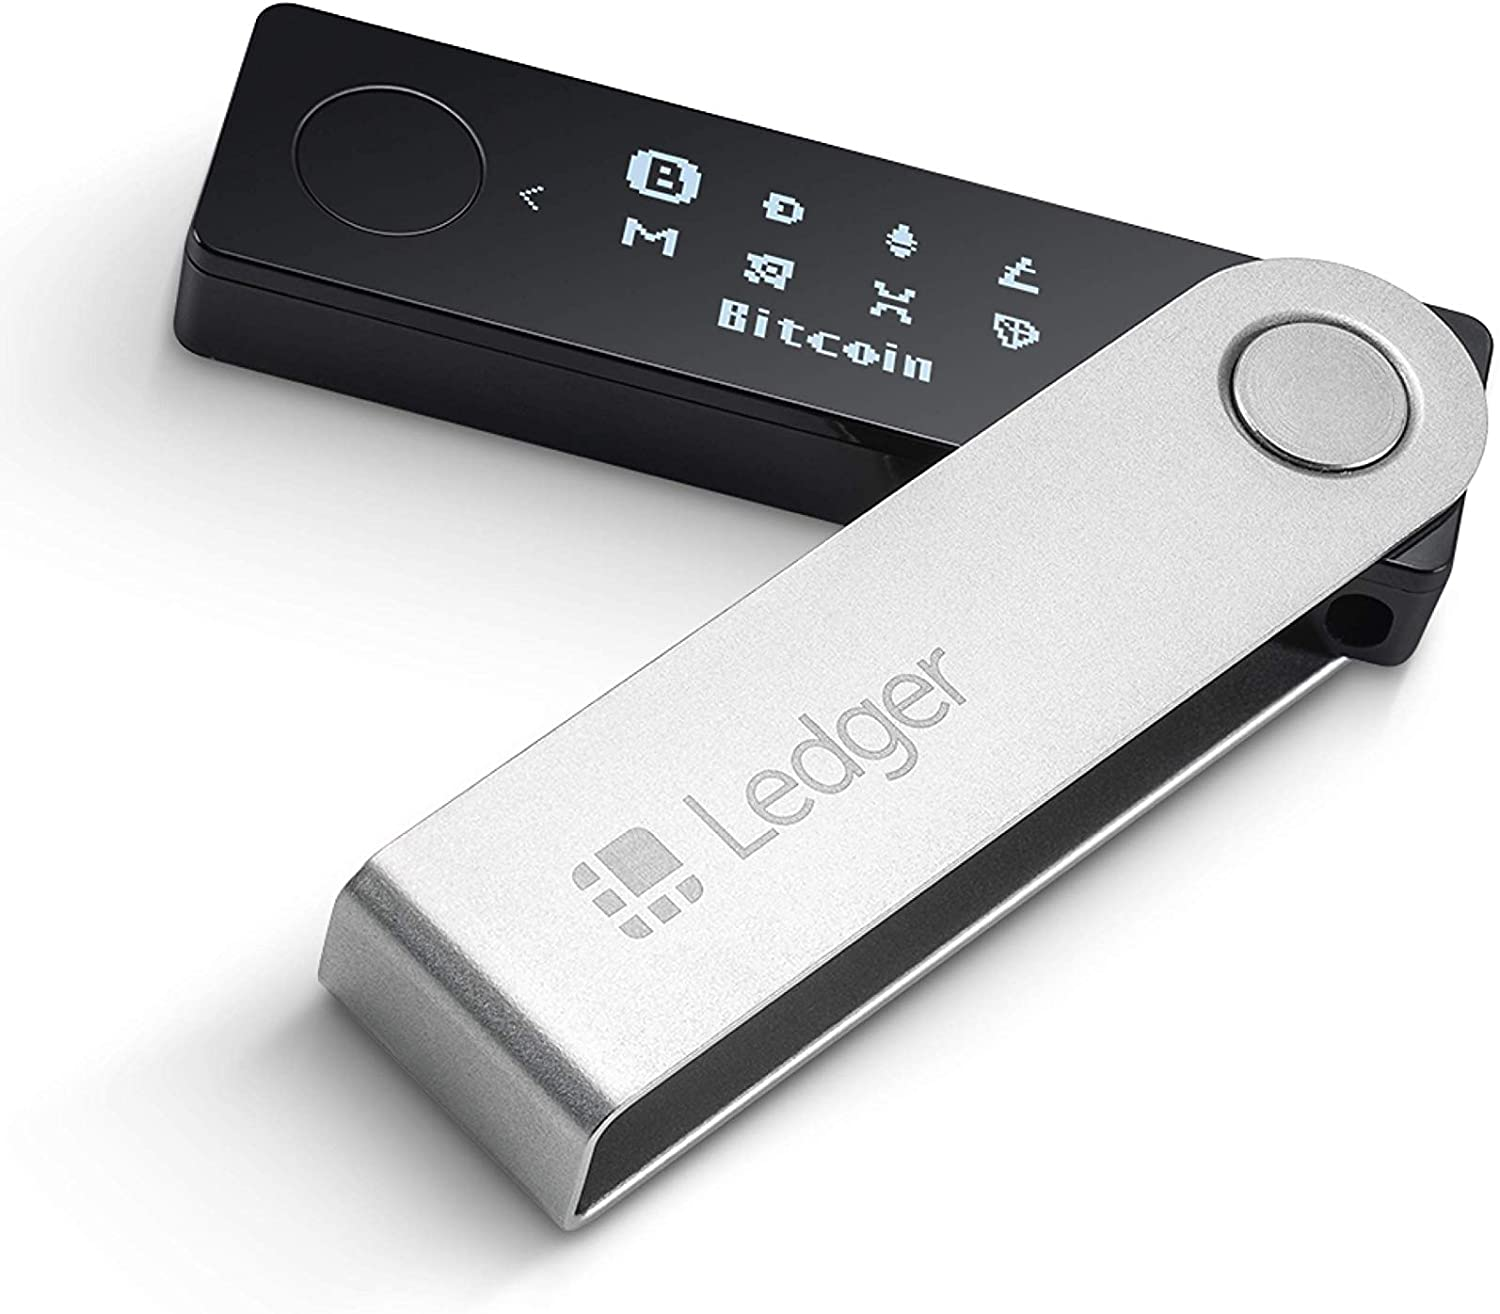
\includegraphics[scale = 0.1]{figures/hardware_wallet.jpg}
    \caption{An Example of a Hardware Wallet\cite{hard}}
    \label{fig:hardware_wallet}
\end{figure}


\subsection{HD Wallets}
For a wallet, we want to generate public and secret key pairs (sk, pk) $\longleftarrow$ $\mathsf{Gen}(1^\kappa)$.

To do this, one approach is to start with a seed that is randomly generated (such as a series of words), then hash the seed with a counter. Note that we cannot use human-generated random words, such as ``I love my dog", because it could be easily stolen.

One commonly used approach is the following. Given a randomly generated \textit{seed}, we can concatenate it with a counter and hash the concatenation to achieve a new secret key. Then, from the secret key, we can generate a public key.
\begin{align*}
H(\text{ctr}\|\text{seed})&\longrightarrow \text{new sk} \\
H(1\|\text{seed}) &\longrightarrow \text{new sk}_0  \\
H(2\|\text{seed}) &\longrightarrow \text{new sk}_1 \\
&\cdots
\end{align*}
